\documentclass[11pt,a4paper]{report}
\usepackage[margin=1in]{geometry}
\usepackage{graphicx}
\usepackage{tikz}
\usepackage{pgfplots}
\usepackage{hyperref}
\usepackage{xcolor}
\usepackage{tabularx}
\usepackage{enumitem}
\usepackage{float}
\usepackage{amsmath}
\usepackage{multicol}

\definecolor{dreamlabblue}{RGB}{0,123,255}
\definecolor{dreamlabgreen}{RGB}{40,167,69}
\definecolor{dreamlabgray}{RGB}{108,117,125}

\title{\textbf{DreamLab Go-To-Market Strategy}\\
\Large AI-Powered Community Engagement Platform for UK Councils}
\author{Marketing \& Strategy Division}
\date{2025-2030 Strategic Plan}

\begin{document}

\maketitle
\tableofcontents

\chapter{Executive Summary}

DreamLab represents a paradigm shift in how UK councils engage with their communities. Our AI-powered platform transforms citizen engagement from reactive service delivery to proactive community collaboration, enabling councils to achieve a 3-5x improvement in engagement metrics while reducing operational costs by 40\%.

\section{Key Value Propositions}
\begin{itemize}
    \item \textbf{Scalable Engagement}: Handle 10x more citizen interactions without increasing staff
    \item \textbf{Data-Driven Insights}: Transform unstructured feedback into actionable intelligence
    \item \textbf{Measurable Impact}: Demonstrate ROI through improved satisfaction scores and cost savings
    \item \textbf{Future-Ready Infrastructure}: Build resilient digital capabilities for evolving citizen expectations
\end{itemize}

\section{Target Market Overview}
Our primary market consists of 317 UK councils managing £60 billion in annual budgets and serving 67 million citizens. We segment this market into three tiers based on population size and digital maturity, with initial focus on Tier 1 and 2 councils representing 80\% of total addressable market value.

\chapter{Market Analysis and Segmentation}

\section{UK Council Landscape}

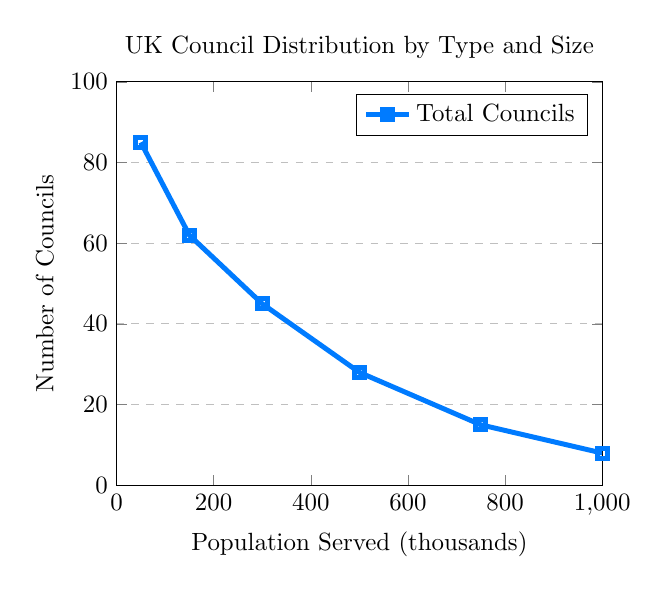
\begin{tikzpicture}[scale=0.9]
\begin{axis}[
    title={UK Council Distribution by Type and Size},
    xlabel={Population Served (thousands)},
    ylabel={Number of Councils},
    xmin=0, xmax=1000,
    ymin=0, ymax=100,
    xtick={0,200,400,600,800,1000},
    ytick={0,20,40,60,80,100},
    legend pos=north east,
    ymajorgrids=true,
    grid style=dashed,
]

\addplot[
    color=dreamlabblue,
    mark=square,
    line width=2pt
    ]
    coordinates {
    (50,85)(150,62)(300,45)(500,28)(750,15)(1000,8)
    };
    \legend{Total Councils}

\end{axis}
\end{tikzpicture}

\section{Market Segmentation Framework}

\subsection{Tier 1: Digital Leaders (15\% of market)}
\begin{itemize}
    \item \textbf{Characteristics}: Large urban councils, >500k population, established digital teams
    \item \textbf{Budget}: £5-10M annual technology spend
    \item \textbf{Needs}: Advanced AI capabilities, integration with existing systems, scalability
    \item \textbf{Decision Process}: 6-9 month evaluation, multiple stakeholders, proof of concept required
\end{itemize}

\subsection{Tier 2: Digital Aspirants (35\% of market)}
\begin{itemize}
    \item \textbf{Characteristics}: Mid-size councils, 100-500k population, emerging digital strategies
    \item \textbf{Budget}: £1-5M annual technology spend
    \item \textbf{Needs}: Easy implementation, proven ROI, staff training and support
    \item \textbf{Decision Process}: 3-6 month evaluation, focused on quick wins
\end{itemize}

\subsection{Tier 3: Digital Explorers (50\% of market)}
\begin{itemize}
    \item \textbf{Characteristics}: Smaller councils, <100k population, limited digital resources
    \item \textbf{Budget}: <£1M annual technology spend
    \item \textbf{Needs}: Cost-effective solutions, minimal IT requirements, shared services
    \item \textbf{Decision Process}: 1-3 month evaluation, price-sensitive
\end{itemize}

\section{Competitive Landscape Analysis}

\begin{table}[H]
\centering
\begin{tabularx}{\textwidth}{|X|X|X|X|X|}
\hline
\textbf{Competitor} & \textbf{Market Share} & \textbf{Strengths} & \textbf{Weaknesses} & \textbf{DreamLab Advantage} \\
\hline
Legacy CRM Systems & 45\% & Established relationships & Poor UX, no AI & Modern AI-first approach \\
\hline
Point Solutions & 30\% & Specific features & Fragmented experience & Unified platform \\
\hline
In-house Development & 20\% & Customization & High cost, slow & Rapid deployment \\
\hline
New Entrants & 5\% & Innovation & Unproven & Validated technology \\
\hline
\end{tabularx}
\end{table}

\chapter{Positioning and Messaging Framework}

\section{Brand Positioning Statement}
DreamLab is the intelligent community engagement platform that empowers UK councils to build stronger, more connected communities through AI-powered insights and automation, transforming how local government understands and serves its citizens.

\section{Messaging Architecture}

\subsection{Core Messages by Audience}

\subsubsection{For Council Leadership}
\begin{itemize}
    \item \textbf{Primary}: "Transform citizen satisfaction while reducing operational costs"
    \item \textbf{Supporting}: 
        \begin{itemize}
            \item Demonstrate measurable community impact
            \item Future-proof your digital infrastructure
            \item Lead in local government innovation
        \end{itemize}
\end{itemize}

\subsubsection{For IT Directors}
\begin{itemize}
    \item \textbf{Primary}: "Enterprise-ready AI platform with seamless integration"
    \item \textbf{Supporting}:
        \begin{itemize}
            \item Cloud-native architecture with 99.9\% uptime
            \item API-first design for existing system integration
            \item GDPR and UK data sovereignty compliance
        \end{itemize}
\end{itemize}

\subsubsection{For Service Managers}
\begin{itemize}
    \item \textbf{Primary}: "Empower your team to deliver exceptional citizen experiences"
    \item \textbf{Supporting}:
        \begin{itemize}
            \item Automate routine inquiries, focus on complex cases
            \item Real-time insights for service improvement
            \item Intuitive tools requiring minimal training
        \end{itemize}
\end{itemize}

\section{Value Proposition Canvas}

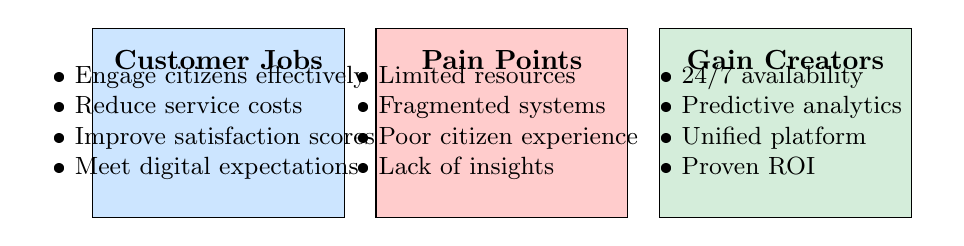
\begin{tikzpicture}[scale=0.8]
    % Customer Jobs
    \draw[fill=dreamlabblue!20] (0,0) rectangle (4,3);
    \node[align=center] at (2,2.5) {\textbf{Customer Jobs}};
    \node[align=left] at (2,1.5) {
        \small
        \begin{tabular}{l}
        • Engage citizens effectively\\
        • Reduce service costs\\
        • Improve satisfaction scores\\
        • Meet digital expectations
        \end{tabular}
    };
    
    % Pain Points
    \draw[fill=red!20] (4.5,0) rectangle (8.5,3);
    \node[align=center] at (6.5,2.5) {\textbf{Pain Points}};
    \node[align=left] at (6.5,1.5) {
        \small
        \begin{tabular}{l}
        • Limited resources\\
        • Fragmented systems\\
        • Poor citizen experience\\
        • Lack of insights
        \end{tabular}
    };
    
    % Gain Creators
    \draw[fill=dreamlabgreen!20] (9,0) rectangle (13,3);
    \node[align=center] at (11,2.5) {\textbf{Gain Creators}};
    \node[align=left] at (11,1.5) {
        \small
        \begin{tabular}{l}
        • 24/7 availability\\
        • Predictive analytics\\
        • Unified platform\\
        • Proven ROI
        \end{tabular}
    };
\end{tikzpicture}

\chapter{Channel Strategy and Tactics}

\section{Multi-Channel Go-to-Market Approach}

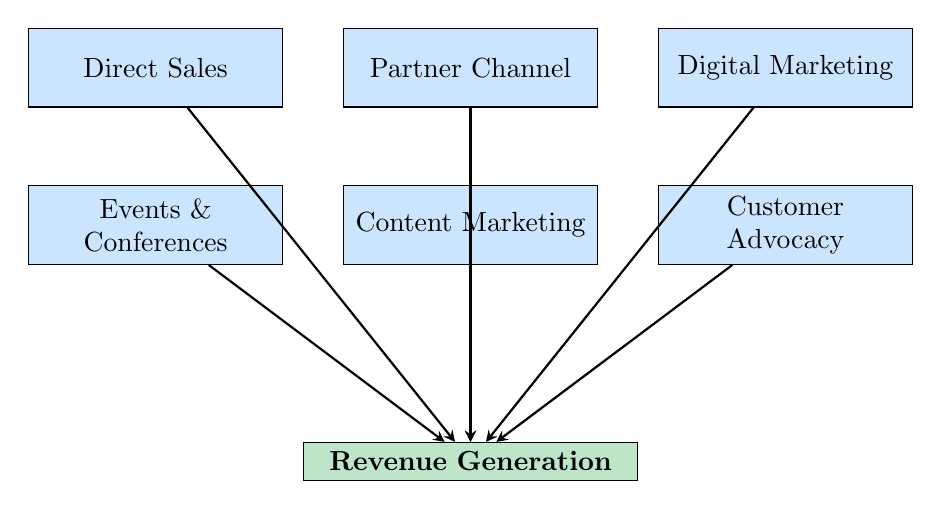
\begin{tikzpicture}[node distance=2cm]
    \tikzstyle{channel} = [rectangle, draw, fill=dreamlabblue!20, text width=3cm, text centered, minimum height=1cm]
    \tikzstyle{arrow} = [thick,->,>=stealth]
    
    \node[channel] (direct) {Direct Sales};
    \node[channel, right of=direct, xshift=2cm] (partner) {Partner Channel};
    \node[channel, right of=partner, xshift=2cm] (digital) {Digital Marketing};
    \node[channel, below of=direct] (events) {Events \& Conferences};
    \node[channel, below of=partner] (content) {Content Marketing};
    \node[channel, below of=digital] (advocacy) {Customer Advocacy};
    
    \node[draw, fill=dreamlabgreen!30, text width=4cm, text centered, below of=content, yshift=-1cm] (revenue) {\textbf{Revenue Generation}};
    
    \draw[arrow] (direct) -- (revenue);
    \draw[arrow] (partner) -- (revenue);
    \draw[arrow] (digital) -- (revenue);
    \draw[arrow] (events) -- (revenue);
    \draw[arrow] (content) -- (revenue);
    \draw[arrow] (advocacy) -- (revenue);
\end{tikzpicture}

\section{Direct Sales Strategy}

\subsection{Sales Team Structure}
\begin{itemize}
    \item \textbf{Enterprise Account Executives} (4): Focus on Tier 1 councils
    \item \textbf{Regional Sales Managers} (8): Cover Tier 2 councils by geography
    \item \textbf{Inside Sales Representatives} (6): Qualify leads and support Tier 3
    \item \textbf{Sales Engineers} (4): Technical demonstrations and POCs
\end{itemize}

\subsection{Sales Process Methodology}

\begin{enumerate}
    \item \textbf{Discovery} (Week 1-2)
        \begin{itemize}
            \item Identify key stakeholders and pain points
            \item Assess current technology landscape
            \item Quantify improvement opportunities
        \end{itemize}
    
    \item \textbf{Solution Design} (Week 3-4)
        \begin{itemize}
            \item Customize demo for specific use cases
            \item Develop ROI model with council data
            \item Align with procurement requirements
        \end{itemize}
    
    \item \textbf{Proof of Concept} (Week 5-8)
        \begin{itemize}
            \item Deploy limited pilot with real data
            \item Measure initial results and feedback
            \item Build internal champion network
        \end{itemize}
    
    \item \textbf{Commercial Negotiation} (Week 9-12)
        \begin{itemize}
            \item Present business case to decision makers
            \item Navigate procurement framework
            \item Finalize terms and implementation plan
        \end{itemize}
\end{enumerate}

\section{Partner Channel Development}

\subsection{Strategic Partner Categories}

\subsubsection{System Integrators}
\begin{itemize}
    \item \textbf{Targets}: Capita, Serco, Sopra Steria
    \item \textbf{Value Proposition}: Add AI capabilities to existing contracts
    \item \textbf{Revenue Share}: 20-30\% of license revenue
\end{itemize}

\subsubsection{Technology Partners}
\begin{itemize}
    \item \textbf{Targets}: Microsoft, AWS, Salesforce
    \item \textbf{Value Proposition}: Complement cloud and CRM investments
    \item \textbf{Go-to-Market}: Joint solutions and marketplace listings
\end{itemize}

\subsubsection{Consultancy Partners}
\begin{itemize}
    \item \textbf{Targets}: PwC, Deloitte, KPMG public sector practices
    \item \textbf{Value Proposition}: Enable digital transformation projects
    \item \textbf{Engagement Model}: Referral fees and implementation services
\end{itemize}

\section{Digital Marketing Strategy}

\subsection{Content Marketing Hub}

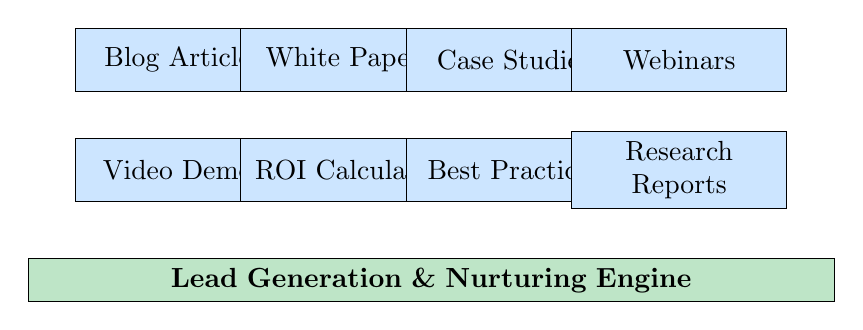
\begin{tikzpicture}[scale=0.7]
    \tikzstyle{content} = [rectangle, draw, fill=dreamlabblue!20, text width=2.5cm, text centered, minimum height=0.8cm]
    
    \node[content] at (0,0) {Blog Articles};
    \node[content] at (3,0) {White Papers};
    \node[content] at (6,0) {Case Studies};
    \node[content] at (9,0) {Webinars};
    \node[content] at (0,-2) {Video Demos};
    \node[content] at (3,-2) {ROI Calculator};
    \node[content] at (6,-2) {Best Practices};
    \node[content] at (9,-2) {Research Reports};
    
    \node[draw, fill=dreamlabgreen!30, text width=10cm, text centered] at (4.5,-4) {\textbf{Lead Generation \& Nurturing Engine}};
\end{tikzpicture}

\subsection{SEO and SEM Strategy}

\subsubsection{Target Keywords}
\begin{multicols}{2}
\begin{itemize}
    \item council citizen engagement platform
    \item local government AI solutions
    \item community consultation software
    \item council digital transformation
    \item citizen experience management
    \item public sector automation
\end{itemize}
\end{multicols}

\subsubsection{Paid Search Campaigns}
\begin{itemize}
    \item \textbf{Budget Allocation}: £50k/month initial investment
    \item \textbf{Target CPC}: £15-25 for high-intent keywords
    \item \textbf{Conversion Goal}: 15\% landing page to demo request
\end{itemize}

\chapter{Sales Funnel and Conversion Metrics}

\section{Customer Acquisition Funnel}

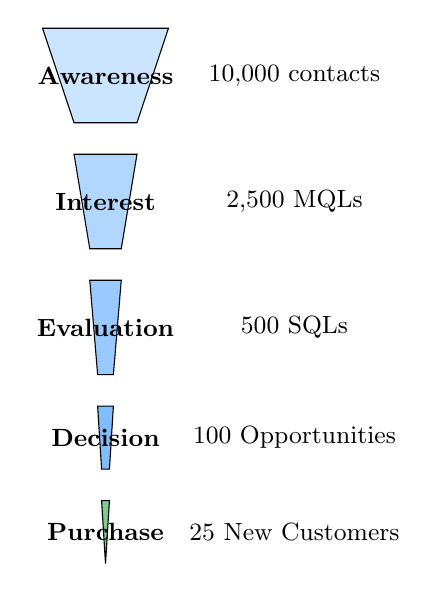
\begin{tikzpicture}[scale=0.8]
    \draw[fill=dreamlabblue!20] (0,0) -- (2,0) -- (1.5,-1.5) -- (0.5,-1.5) -- cycle;
    \node at (1,-0.75) {\small \textbf{Awareness}};
    \node at (4,-0.75) {\small 10,000 contacts};
    
    \draw[fill=dreamlabblue!30] (0.5,-2) -- (1.5,-2) -- (1.25,-3.5) -- (0.75,-3.5) -- cycle;
    \node at (1,-2.75) {\small \textbf{Interest}};
    \node at (4,-2.75) {\small 2,500 MQLs};
    
    \draw[fill=dreamlabblue!40] (0.75,-4) -- (1.25,-4) -- (1.125,-5.5) -- (0.875,-5.5) -- cycle;
    \node at (1,-4.75) {\small \textbf{Evaluation}};
    \node at (4,-4.75) {\small 500 SQLs};
    
    \draw[fill=dreamlabblue!50] (0.875,-6) -- (1.125,-6) -- (1.0625,-7) -- (0.9375,-7) -- cycle;
    \node at (1,-6.5) {\small \textbf{Decision}};
    \node at (4,-6.5) {\small 100 Opportunities};
    
    \draw[fill=dreamlabgreen!60] (0.9375,-7.5) -- (1.0625,-7.5) -- (1,-8.5) -- cycle;
    \node at (1,-8) {\small \textbf{Purchase}};
    \node at (4,-8) {\small 25 New Customers};
\end{tikzpicture}

\section{Conversion Rate Optimization}

\subsection{Stage-by-Stage Metrics}
\begin{table}[H]
\centering
\begin{tabularx}{\textwidth}{|X|c|c|c|c|}
\hline
\textbf{Funnel Stage} & \textbf{Target Rate} & \textbf{Current Rate} & \textbf{Benchmark} & \textbf{Improvement Actions} \\
\hline
Visitor to Lead & 5\% & 3.2\% & 4\% & Enhanced content offers \\
\hline
Lead to MQL & 25\% & 18\% & 20\% & Lead scoring optimization \\
\hline
MQL to SQL & 20\% & 15\% & 18\% & Better qualification criteria \\
\hline
SQL to Opportunity & 40\% & 35\% & 35\% & Improved demos \\
\hline
Opportunity to Close & 25\% & 20\% & 22\% & ROI tools, references \\
\hline
\end{tabularx}
\end{table}

\section{Customer Acquisition Cost (CAC) Model}

\begin{align}
\text{CAC} &= \frac{\text{Total Sales \& Marketing Costs}}{\text{New Customers Acquired}} \\
&= \frac{£2,400,000}{25} = £96,000
\end{align}

\subsection{CAC Payback Analysis}
\begin{itemize}
    \item \textbf{Average Contract Value}: £150,000/year
    \item \textbf{Gross Margin}: 75\%
    \item \textbf{Payback Period}: 10.2 months
    \item \textbf{LTV:CAC Ratio}: 4.7:1
\end{itemize}

\chapter{Pricing Strategy and Packaging}

\section{Value-Based Pricing Framework}

\subsection{Pricing Principles}
\begin{enumerate}
    \item \textbf{Align with Value Delivery}: Price based on citizen engagement outcomes
    \item \textbf{Scalable Model}: Growing councils shouldn't be penalized
    \item \textbf{Predictable Costs}: Annual contracts with clear tier boundaries
    \item \textbf{ROI Justification}: Demonstrate 3:1 return within first year
\end{enumerate}

\section{Product Packaging Tiers}

\begin{table}[H]
\centering
\begin{tabularx}{\textwidth}{|X|X|X|X|}
\hline
\textbf{Package} & \textbf{Essentials} & \textbf{Professional} & \textbf{Enterprise} \\
\hline
\textbf{Target Segment} & Tier 3 Councils & Tier 2 Councils & Tier 1 Councils \\
\hline
\textbf{Citizens Served} & Up to 100k & 100k - 500k & 500k+ \\
\hline
\textbf{Base Price} & £35k/year & £75k/year & £150k/year \\
\hline
\textbf{AI Interactions} & 50k/month & 250k/month & Unlimited \\
\hline
\textbf{Users} & 25 & 100 & Unlimited \\
\hline
\textbf{Integrations} & 3 & 10 & Unlimited \\
\hline
\textbf{Support} & Business hours & Extended hours & 24/7 + CSM \\
\hline
\textbf{Features} & 
Core engagement tools &
Advanced analytics, API access &
Custom ML models, white-label \\
\hline
\end{tabularx}
\end{table}

\section{Pricing Modifiers and Add-ons}

\subsection{Volume Discounts}
\begin{itemize}
    \item 3-year commitment: 15\% discount
    \item 5-year commitment: 25\% discount
    \item Multi-council (shared services): 20\% discount per additional council
\end{itemize}

\subsection{Professional Services}
\begin{itemize}
    \item \textbf{Implementation Package}: £25k-50k based on complexity
    \item \textbf{Custom Integration}: £1,500/day
    \item \textbf{Training Programs}: £5k for standard, £15k for train-the-trainer
    \item \textbf{Ongoing Consultancy}: £1,200/day
\end{itemize}

\chapter{Launch Plan and Timeline}

\section{Phased Market Entry Strategy}

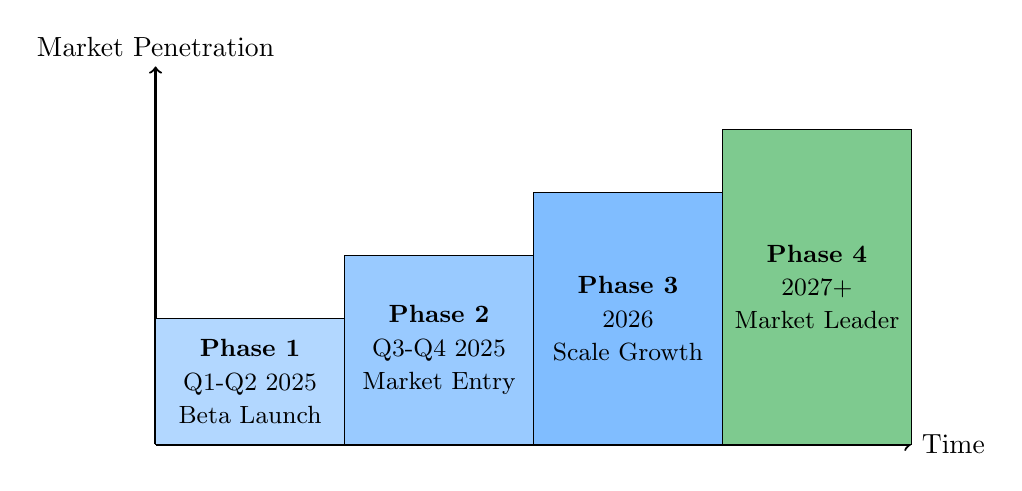
\begin{tikzpicture}[scale=0.8]
    \draw[thick,->] (0,0) -- (12,0) node[right] {Time};
    \draw[thick,->] (0,0) -- (0,6) node[above] {Market Penetration};
    
    % Phase 1
    \draw[fill=dreamlabblue!30] (0,0) rectangle (3,2);
    \node[align=center] at (1.5,1) {\small \textbf{Phase 1}\\\small Q1-Q2 2025\\\small Beta Launch};
    
    % Phase 2
    \draw[fill=dreamlabblue!40] (3,0) rectangle (6,3);
    \node[align=center] at (4.5,1.5) {\small \textbf{Phase 2}\\\small Q3-Q4 2025\\\small Market Entry};
    
    % Phase 3
    \draw[fill=dreamlabblue!50] (6,0) rectangle (9,4);
    \node[align=center] at (7.5,2) {\small \textbf{Phase 3}\\\small 2026\\\small Scale Growth};
    
    % Phase 4
    \draw[fill=dreamlabgreen!60] (9,0) rectangle (12,5);
    \node[align=center] at (10.5,2.5) {\small \textbf{Phase 4}\\\small 2027+\\\small Market Leader};
\end{tikzpicture}

\section{Phase 1: Beta Launch (Q1-Q2 2025)}

\subsection{Objectives}
\begin{itemize}
    \item Recruit 5-7 beta councils across different tiers
    \item Validate product-market fit and pricing model
    \item Generate initial case studies and testimonials
    \item Refine go-to-market messaging based on feedback
\end{itemize}

\subsection{Key Activities}
\begin{itemize}
    \item \textbf{Week 1-4}: Beta partner recruitment and onboarding
    \item \textbf{Week 5-12}: Deployment and initial usage monitoring
    \item \textbf{Week 13-20}: Feedback collection and product iteration
    \item \textbf{Week 21-24}: Case study development and launch preparation
\end{itemize}

\section{Phase 2: Market Entry (Q3-Q4 2025)}

\subsection{Launch Campaign Elements}
\begin{enumerate}
    \item \textbf{PR Blitz}
        \begin{itemize}
            \item Exclusive with The Guardian Public Leaders Network
            \item Coverage in LocalGov, PublicTechnology, UKAuthority
            \item Thought leadership articles by CEO
        \end{itemize}
    
    \item \textbf{Launch Events}
        \begin{itemize}
            \item Virtual launch event for 500+ council leaders
            \item Regional roadshow in 6 major cities
            \item Presence at LocalGov Expo and Socitm Conference
        \end{itemize}
    
    \item \textbf{Digital Campaign}
        \begin{itemize}
            \item Targeted LinkedIn campaign to 10k+ decision makers
            \item Google Ads with £100k launch budget
            \item Email nurture series to qualified database
        \end{itemize}
\end{enumerate}

\section{Phase 3: Scale Growth (2026)}

\subsection{Growth Targets}
\begin{itemize}
    \item Achieve 50 paying customers
    \item £7.5M ARR
    \item 90\% customer retention rate
    \item Launch partner program with 10 active partners
\end{itemize}

\subsection{Market Expansion}
\begin{itemize}
    \item Expand from England to full UK coverage
    \item Launch specialized solutions for specific council types
    \item Introduce premium AI capabilities for advanced use cases
    \item Begin international market assessment (Ireland, Australia)
\end{itemize}

\chapter{Partnership and Ecosystem Strategy}

\section{Ecosystem Development Framework}

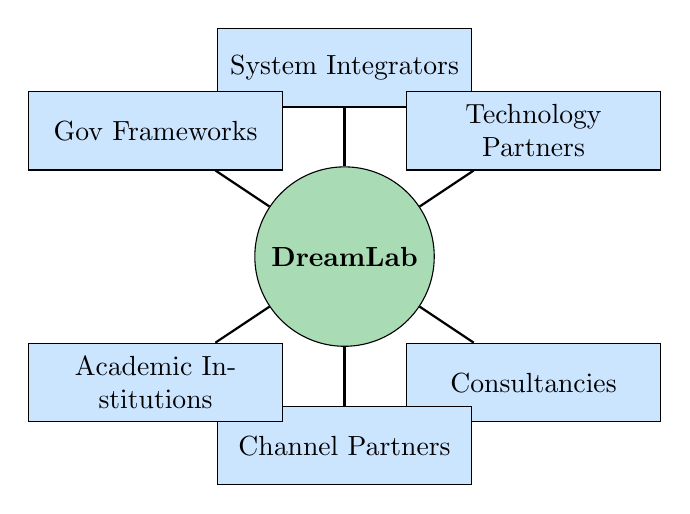
\begin{tikzpicture}[scale=0.8]
    \tikzstyle{partner} = [rectangle, draw, fill=dreamlabblue!20, text width=3cm, text centered, minimum height=1cm]
    \tikzstyle{dreamlab} = [circle, draw, fill=dreamlabgreen!40, text width=2cm, text centered, minimum height=2cm]
    
    \node[dreamlab] (center) {\textbf{DreamLab}};
    
    \node[partner] (si) at (0,3) {System Integrators};
    \node[partner] (tech) at (3,2) {Technology Partners};
    \node[partner] (consult) at (3,-2) {Consultancies};
    \node[partner] (channel) at (0,-3) {Channel Partners};
    \node[partner] (academic) at (-3,-2) {Academic Institutions};
    \node[partner] (gov) at (-3,2) {Gov Frameworks};
    
    \draw[thick] (center) -- (si);
    \draw[thick] (center) -- (tech);
    \draw[thick] (center) -- (consult);
    \draw[thick] (center) -- (channel);
    \draw[thick] (center) -- (academic);
    \draw[thick] (center) -- (gov);
\end{tikzpicture}

\section{Strategic Partnership Priorities}

\subsection{Government Procurement Frameworks}
\begin{itemize}
    \item \textbf{G-Cloud 14}: Submit application by Q2 2025
    \item \textbf{Digital Outcomes and Specialists 6}: Qualify for Lot 1 and 2
    \item \textbf{Crown Commercial Service}: Achieve preferred supplier status
    \item \textbf{Local Government Association}: Endorsement and promotion
\end{itemize}

\subsection{Technology Integration Partners}

\subsubsection{Priority Integrations}
\begin{table}[H]
\centering
\begin{tabularx}{\textwidth}{|X|X|X|X|}
\hline
\textbf{Partner} & \textbf{Integration Type} & \textbf{Value Proposition} & \textbf{Timeline} \\
\hline
Microsoft & Azure AD, Teams & Seamless authentication and collaboration & Q2 2025 \\
\hline
Salesforce & Public Sector Cloud & Enhance CRM capabilities & Q3 2025 \\
\hline
Oracle & Finance systems & Budget and planning insights & Q4 2025 \\
\hline
Civica & Service delivery & End-to-end citizen journey & Q1 2026 \\
\hline
\end{tabularx}
\end{table}

\section{Partner Program Structure}

\subsection{Partner Tiers and Benefits}

\begin{enumerate}
    \item \textbf{Certified Partner}
        \begin{itemize}
            \item Requirements: 2 certified staff, 1 customer reference
            \item Benefits: 15\% revenue share, lead sharing, co-marketing
        \end{itemize}
    
    \item \textbf{Silver Partner}
        \begin{itemize}
            \item Requirements: 5 certified staff, 3 implementations
            \item Benefits: 20\% revenue share, dedicated support, MDF
        \end{itemize}
    
    \item \textbf{Gold Partner}
        \begin{itemize}
            \item Requirements: 10 certified staff, 10 implementations
            \item Benefits: 25\% revenue share, strategic planning, joint GTM
        \end{itemize}
\end{enumerate}

\subsection{Partner Enablement Program}
\begin{itemize}
    \item \textbf{Training}: 3-day certification program with annual recertification
    \item \textbf{Sales Tools}: Demo environments, battle cards, ROI calculators
    \item \textbf{Marketing Support}: Co-branded materials, lead generation campaigns
    \item \textbf{Technical Resources}: API documentation, integration guides, sandbox
\end{itemize}

\chapter{Customer Success and Retention Strategy}

\section{Customer Success Framework}

\subsection{Success Metrics and KPIs}
\begin{itemize}
    \item \textbf{Adoption Rate}: 80\% of licensed users active within 90 days
    \item \textbf{Feature Utilization}: Progressive adoption of advanced features
    \item \textbf{Business Outcomes}: Measurable improvement in citizen satisfaction
    \item \textbf{Health Score}: Composite metric predicting renewal probability
\end{itemize}

\section{Customer Journey Mapping}

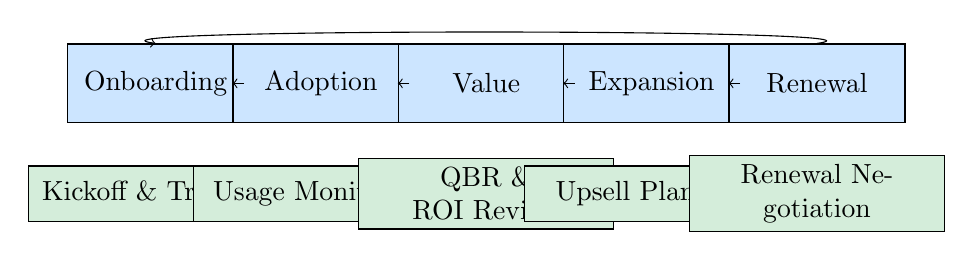
\begin{tikzpicture}[scale=0.7]
    \tikzstyle{stage} = [rectangle, draw, fill=dreamlabblue!20, text width=2cm, text centered, minimum height=1cm]
    \tikzstyle{action} = [rectangle, draw, fill=dreamlabgreen!20, text width=3cm, text centered, minimum height=0.7cm]
    
    % Stages
    \node[stage] (onboard) at (0,0) {Onboarding};
    \node[stage] (adopt) at (3,0) {Adoption};
    \node[stage] (value) at (6,0) {Value};
    \node[stage] (expand) at (9,0) {Expansion};
    \node[stage] (renew) at (12,0) {Renewal};
    
    % Actions
    \node[action] (a1) at (0,-2) {Kickoff \& Training};
    \node[action] (a2) at (3,-2) {Usage Monitoring};
    \node[action] (a3) at (6,-2) {QBR \& ROI Review};
    \node[action] (a4) at (9,-2) {Upsell Planning};
    \node[action] (a5) at (12,-2) {Renewal Negotiation};
    
    % Connections
    \draw[->] (onboard) -- (adopt);
    \draw[->] (adopt) -- (value);
    \draw[->] (value) -- (expand);
    \draw[->] (expand) -- (renew);
    \draw[->] (renew.north) .. controls (14,1) and (-2,1) .. (onboard.north);
\end{tikzpicture}

\section{Retention and Growth Programs}

\subsection{Quarterly Business Reviews (QBRs)}
\begin{itemize}
    \item Executive-level engagement showcasing ROI and impact
    \item Roadmap alignment and feature request prioritization
    \item Success story documentation for internal champions
    \item Identification of expansion opportunities
\end{itemize}

\subsection{User Community Building}
\begin{itemize}
    \item \textbf{DreamLab User Forum}: Online community for peer learning
    \item \textbf{Annual Conference}: DreamLab Summit for networking and best practices
    \item \textbf{Regional Meetups}: Quarterly gatherings in major regions
    \item \textbf{Innovation Awards}: Recognize exceptional implementations
\end{itemize}

\subsection{Advocacy Program}
\begin{itemize}
    \item \textbf{Reference Customers}: Incentivized program for case studies
    \item \textbf{Speaking Opportunities}: Platform at industry events
    \item \textbf{Advisory Board}: Strategic input from key customers
    \item \textbf{Beta Access}: Early feature access for engaged customers
\end{itemize}

\chapter{Revenue Projections and Targets}

\section{5-Year Revenue Model}

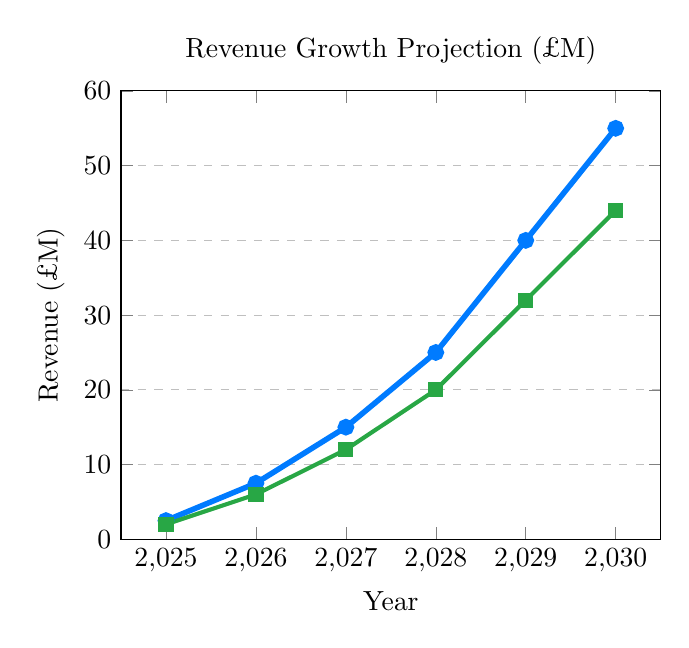
\begin{tikzpicture}
\begin{axis}[
    title={Revenue Growth Projection (£M)},
    xlabel={Year},
    ylabel={Revenue (£M)},
    xmin=2024.5, xmax=2030.5,
    ymin=0, ymax=60,
    xtick={2025,2026,2027,2028,2029,2030},
    ytick={0,10,20,30,40,50,60},
    legend pos=north west,
    ymajorgrids=true,
    grid style=dashed,
]

\addplot[
    color=dreamlabblue,
    mark=*,
    line width=2pt
    ]
    coordinates {
    (2025,2.5)(2026,7.5)(2027,15)(2028,25)(2029,40)(2030,55)
    };
\addlegend{Total Revenue}

\addplot[
    color=dreamlabgreen,
    mark=square*,
    line width=1.5pt
    ]
    coordinates {
    (2025,2)(2026,6)(2027,12)(2028,20)(2029,32)(2030,44)
    };
\addlegend{Recurring Revenue}

\end{axis}
\end{tikzpicture}

\section{Customer Acquisition Targets}

\begin{table}[H]
\centering
\begin{tabularx}{\textwidth}{|c|c|c|c|c|c|}
\hline
\textbf{Year} & \textbf{New Customers} & \textbf{Total Customers} & \textbf{Avg. ACV} & \textbf{Churn Rate} & \textbf{NRR} \\
\hline
2025 & 15 & 15 & £150k & 5\% & 110\% \\
\hline
2026 & 35 & 49 & £155k & 8\% & 115\% \\
\hline
2027 & 60 & 105 & £160k & 10\% & 120\% \\
\hline
2028 & 80 & 175 & £165k & 10\% & 125\% \\
\hline
2029 & 100 & 258 & £170k & 12\% & 125\% \\
\hline
2030 & 120 & 346 & £175k & 12\% & 130\% \\
\hline
\end{tabularx}
\end{table}

\section{Market Share Projections}

\subsection{Total Addressable Market (TAM)}
\begin{itemize}
    \item \textbf{UK Council Technology Spend}: £2.5B annually
    \item \textbf{Citizen Engagement Segment}: £300M (12\% of total)
    \item \textbf{Serviceable Addressable Market}: £180M (60\% of segment)
    \item \textbf{Target Market Share by 2030}: 30\% (£54M)
\end{itemize}

\chapter{Marketing Mix and Budget Allocation}

\section{Marketing Investment Framework}

\begin{table}[H]
\centering
\begin{tabularx}{\textwidth}{|X|c|c|c|}
\hline
\textbf{Category} & \textbf{\% of Revenue} & \textbf{2025 Budget} & \textbf{Key Metrics} \\
\hline
Digital Marketing & 8\% & £200k & CPL: £50, MQL: 2,500 \\
\hline
Content Marketing & 6\% & £150k & Content pieces: 100, Engagement: 25k \\
\hline
Events \& Conferences & 10\% & £250k & Leads: 500, Meetings: 150 \\
\hline
Partner Marketing & 4\% & £100k & Partner leads: 300 \\
\hline
PR \& Analyst Relations & 5\% & £125k & Coverage: 50 articles, Mentions: 200 \\
\hline
Sales Enablement & 7\% & £175k & Win rate improvement: 5\% \\
\hline
\textbf{Total} & \textbf{40\%} & \textbf{£1M} & \textbf{ROI: 5:1} \\
\hline
\end{tabularx}
\end{table}

\section{Campaign Calendar and Major Initiatives}

\subsection{Q1 2025: Foundation Building}
\begin{itemize}
    \item Launch new website with conversion optimization
    \item Develop core content library (10 white papers, 20 case studies)
    \item Establish analyst relationships (Gartner, Forrester)
    \item Beta customer recruitment campaign
\end{itemize}

\subsection{Q2 2025: Market Education}
\begin{itemize}
    \item Thought leadership campaign on AI in government
    \item Webinar series: "Future of Citizen Engagement"
    \item LocalGov Digital conference sponsorship
    \item ROI calculator and assessment tools launch
\end{itemize}

\subsection{Q3 2025: Launch Acceleration}
\begin{itemize}
    \item Major product launch event and PR campaign
    \item Customer success story roadshow
    \item Digital advertising blitz (£100k spend)
    \item Partner recruitment drive
\end{itemize}

\subsection{Q4 2025: Market Penetration}
\begin{itemize}
    \item Account-based marketing to top 50 councils
    \item Awards submission campaign
    \item Year-end budget capture campaigns
    \item Customer advisory board formation
\end{itemize}

\chapter{Competitive Differentiation Strategy}

\section{Unique Value Propositions}

\subsection{Technology Differentiation}
\begin{itemize}
    \item \textbf{AI-First Architecture}: Purpose-built for government use cases
    \item \textbf{UK Data Sovereignty}: All data processed within UK borders
    \item \textbf{Ethical AI Framework}: Transparent, auditable decision-making
    \item \textbf{No-Code Customization}: Council staff can adapt without IT
\end{itemize}

\subsection{Business Model Innovation}
\begin{itemize}
    \item \textbf{Outcome-Based Pricing}: Tie fees to citizen satisfaction improvements
    \item \textbf{Shared Success Model}: Reinvest savings into community programs
    \item \textbf{Open Ecosystem}: APIs for local innovation and startups
    \item \textbf{Continuous Innovation}: Quarterly feature releases based on feedback
\end{itemize}

\section{Competitive Battle Cards}

\subsection{Against Legacy Vendors}
\begin{table}[H]
\centering
\begin{tabularx}{\textwidth}{|X|X|X|}
\hline
\textbf{Their Claim} & \textbf{Reality} & \textbf{Our Response} \\
\hline
"Proven and stable" & Outdated technology, poor UX & Modern AI delivers 10x better outcomes \\
\hline
"Integrated suite" & Vendor lock-in, expensive & Open platform with best-of-breed approach \\
\hline
"Industry experience" & Resistant to innovation & Fresh perspective with council input \\
\hline
\end{tabularx}
\end{table}

\subsection{Against New Entrants}
\begin{table}[H]
\centering
\begin{tabularx}{\textwidth}{|X|X|X|}
\hline
\textbf{Their Claim} & \textbf{Reality} & \textbf{Our Response} \\
\hline
"Latest technology" & Unproven at scale & Enterprise-ready with security focus \\
\hline
"Agile and fast" & Limited resources & Backed by major investors, sustainable \\
\hline
"Cheaper solution" & Hidden costs, limited features & True TCO lower with better outcomes \\
\hline
\end{tabularx}
\end{table}

\chapter{Risk Mitigation and Contingency Planning}

\section{Market Risk Assessment}

\begin{table}[H]
\centering
\begin{tabularx}{\textwidth}{|X|c|c|X|}
\hline
\textbf{Risk Factor} & \textbf{Probability} & \textbf{Impact} & \textbf{Mitigation Strategy} \\
\hline
Budget constraints & High & High & Flexible pricing, phased deployment, ROI tools \\
\hline
Slow adoption & Medium & High & Strong change management, training programs \\
\hline
Competition & High & Medium & Continuous innovation, customer lock-in \\
\hline
Regulation changes & Low & High & Compliance team, government relations \\
\hline
Technology failure & Low & High & Robust testing, gradual rollouts, SLAs \\
\hline
\end{tabularx}
\end{table}

\section{Contingency Scenarios}

\subsection{Scenario 1: Economic Downturn}
\begin{itemize}
    \item \textbf{Trigger}: Government spending cuts of 20\%+
    \item \textbf{Response}: 
        \begin{itemize}
            \item Shift to efficiency-focused messaging
            \item Introduce budget-relief pricing options
            \item Partner with councils for shared services
            \item Focus on quick-win implementations
        \end{itemize}
\end{itemize}

\subsection{Scenario 2: Major Competitor Entry}
\begin{itemize}
    \item \textbf{Trigger}: Global tech giant enters market
    \item \textbf{Response}:
        \begin{itemize}
            \item Accelerate feature development
            \item Lock in key accounts with long-term contracts
            \item Emphasize local expertise and support
            \item Consider strategic partnerships or acquisition
        \end{itemize}
\end{itemize}

\chapter{Success Metrics and KPIs}

\section{Go-to-Market Scorecard}

\begin{table}[H]
\centering
\begin{tabularx}{\textwidth}{|X|X|c|c|}
\hline
\textbf{Metric Category} & \textbf{KPI} & \textbf{2025 Target} & \textbf{Measurement Frequency} \\
\hline
\multirow{3}{*}{Pipeline} & Pipeline Value & £15M & Weekly \\
& Pipeline Velocity & 90 days & Monthly \\
& Win Rate & 25\% & Monthly \\
\hline
\multirow{3}{*}{Revenue} & New ARR & £2.5M & Monthly \\
& Expansion Revenue & 15\% & Quarterly \\
& Revenue per Employee & £125k & Quarterly \\
\hline
\multirow{3}{*}{Customer} & NPS Score & 50+ & Quarterly \\
& Customer Retention & 95\% & Annual \\
& Time to Value & 30 days & Per customer \\
\hline
\multirow{3}{*}{Marketing} & Marketing Qualified Leads & 2,500 & Monthly \\
& Cost per Lead & £50 & Monthly \\
& Content Engagement & 25k/month & Monthly \\
\hline
\end{tabularx}
\end{table}

\section{Executive Dashboard Design}

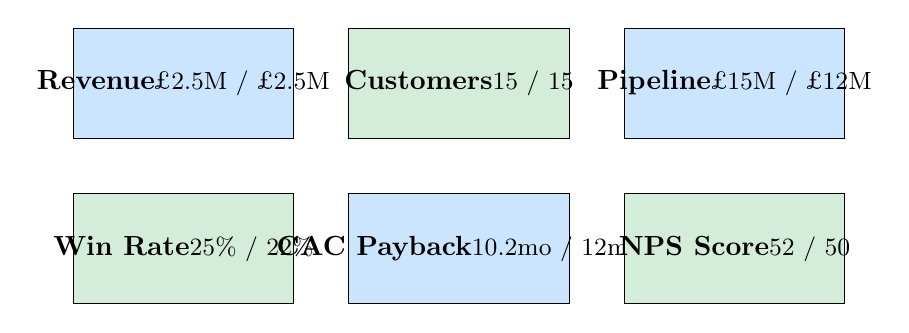
\begin{tikzpicture}[scale=0.7]
    \draw[fill=dreamlabblue!20] (0,0) rectangle (4,2);
    \node at (2,1) {\textbf{Revenue}\\\small £2.5M / £2.5M};
    
    \draw[fill=dreamlabgreen!20] (5,0) rectangle (9,2);
    \node at (7,1) {\textbf{Customers}\\\small 15 / 15};
    
    \draw[fill=dreamlabblue!20] (10,0) rectangle (14,2);
    \node at (12,1) {\textbf{Pipeline}\\\small £15M / £12M};
    
    \draw[fill=dreamlabgreen!20] (0,-3) rectangle (4,-1);
    \node at (2,-2) {\textbf{Win Rate}\\\small 25\% / 22\%};
    
    \draw[fill=dreamlabblue!20] (5,-3) rectangle (9,-1);
    \node at (7,-2) {\textbf{CAC Payback}\\\small 10.2mo / 12mo};
    
    \draw[fill=dreamlabgreen!20] (10,-3) rectangle (14,-1);
    \node at (12,-2) {\textbf{NPS Score}\\\small 52 / 50};
\end{tikzpicture}

\chapter{Conclusion and Next Steps}

\section{Strategic Imperatives for Success}

\subsection{Immediate Actions (Next 30 Days)}
\begin{enumerate}
    \item Finalize beta partner agreements with 5 councils
    \item Complete sales team hiring and training program
    \item Launch digital marketing infrastructure and campaigns
    \item Establish key technology partnerships
    \item Develop initial content library and sales tools
\end{enumerate}

\subsection{Critical Success Factors}
\begin{itemize}
    \item \textbf{Product Excellence}: Deliver measurable value within 30 days
    \item \textbf{Customer Obsession}: Build deep relationships with early adopters
    \item \textbf{Market Education}: Position AI as enabler, not replacement
    \item \textbf{Ecosystem Development}: Create network effects through partnerships
    \item \textbf{Financial Discipline}: Maintain CAC:LTV ratio above 1:3
\end{itemize}

\section{Long-Term Vision}

By 2030, DreamLab will be the recognized leader in government citizen engagement technology, powering meaningful connections between 200+ councils and 40 million UK citizens. Our success will be measured not just in revenue, but in the transformation of public service delivery and the strengthening of democratic participation at the local level.

\subsection{Market Leadership Indicators}
\begin{itemize}
    \item 30\% market share in UK council engagement platforms
    \item £55M+ annual recurring revenue
    \item 95\%+ customer retention rate
    \item International expansion to 5+ countries
    \item Recognition as category-defining solution
\end{itemize}

\section{Investment in Future Growth}

\subsection{Innovation Roadmap}
\begin{itemize}
    \item \textbf{2025}: Core platform and UK market entry
    \item \textbf{2026}: Advanced AI capabilities and partner ecosystem
    \item \textbf{2027}: Vertical solutions for specific service areas
    \item \textbf{2028}: International expansion and platform extensions
    \item \textbf{2029}: Next-generation predictive governance tools
    \item \textbf{2030}: Global leader in government technology
\end{itemize}

\end{document}